\chapter{Introducción al Análisis Exploratorio de Datos}
\noindent
Para entender la estructura de los datos, el Análisis Exploratorio de Datos (AED) se desarrolla:
\begin{itemize}
    \item Descubriendo la estructura subyacente.
    \item Detectando las variables importantes.
    \item Detectando datos anómalos (\textit{outliers}).
    \item Comprobando las hipótesis subyacentes a un análisis.
    \item Desarrollando modelos \textit{ad hoc}.
\end{itemize}

\noindent
Mientras que la \textbf{Estadística descriptiva} tiene la finalidad de resumir conjuntos de datos aportando medidas o estadísticos y la \textbf{Estadística gráfica} es un conjunto de técnicas para mostrar y caracterizar los datos, el \textbf{Análisis Exploratorio de Datos} es una metodología para estudiar la estructura de los datos, basada en técnicas que permiten manejar el conjunto completo de datos para poner de manifiesto su estructura, no para mostrarlos simplemente.\\ 

\noindent
El estudio de los datos debe abordarse desde la filosofía exploratoria:
\begin{description}
    \item [Excepticismo.] El investigador debe adoptar una postura escéptica respecto a las medidas que sintetizan los datos, puesto que pueden ocultar o malinterpretar ciertos aspectos de los datos.
    \item [Apertura.] El investigador debe estar abierto a nuevos modelos no previstos, que pueden surgir al realizar el AED.
\end{description}

\noindent
A modo de resumen, podemos decir que:
\begin{description}
    \item [Estadística clásica.] A partir de los datos, se presupone un modelo basado en hipótesis (linealidad, normalidad, \ldots) y el análisis suele basarse en la estimación y contraste de los parámetros del modelo. Se basa en realizar resúmenes de datos.
    \item [Estadística bayesiana.] Además de lo anterior, se suelen imponer hipótesis sobre la distribución a priori de los parámetros.
    \item [AED.]  A partir de los datos, el análisis se basa en una metodología para estudiar la estructura, patrones y anomalías. A partir de la información se \textbf{decide} el modelo más apropiado, sin asumir hipótesis previas. Se basa en tratar de usar todos los datos, utilizando para ello gráficas.

        El AED complementa la Estadística tradicional, pero es una metodología que no tiene por qué conducir a la estimación de modelos.
\end{description}

\begin{ejemplo}
    ¿Alguna vez has escuchado que la esperanza de vida en la Edad Media era de 30 años? ¿Realmente era raro superar los 40 años de edad?\\

    \noindent
    Este es uno de los más famosos errores en un análisis estadístico. Contamos con los siguientes datos de cuántas muertes se corresponden a cada grupo de edad en la Edad Media para un total de 1000 muertes:
    \begin{table}[H]
        \centering
        \renewcommand{\arraystretch}{1.2}
        \begin{tabular}{c c c}
            \textbf{Grupo de Edad} & \textbf{Edad Media} & \textbf{Muertes} \\
            \hline
            0      & 0.5  & 200 \\
            1--4   & 2.5  & 150 \\
            5--9   & 7.5  & 50  \\
            10--14 & 12.5 & 30  \\
            15--19 & 17.5 & 30  \\
            20--24 & 22.5 & 35  \\
            25--29 & 27.5 & 35  \\
            30--34 & 32.5 & 35  \\
            35--39 & 37.5 & 40  \\
            40--44 & 42.5 & 40  \\
            45--49 & 47.5 & 40  \\
            50--54 & 52.5 & 45  \\
            55--59 & 57.5 & 45  \\
            60--64 & 62.5 & 60  \\
            65--69 & 67.5 & 65  \\
            70--74 & 72.5 & 60  \\
            75--79 & 77.5 & 30  \\
            80+    & 82.5 & 10  \\
        \end{tabular}
        \caption{Datos demográficos ordenados por cohorte de edad en la Edad Media.}
    \end{table}
    \noindent
    A partir de ellos, si queremos calcular cuál es la edad más probable a la que se moría una persona, lo primero que se nos ocurre es calcular la esperanza de edad media de defunción. Hagámoslo en R:
    \begin{figure}[H]
    \begin{minted}{r}
library(ggplot2)
library(dplyr)

# 1. Definir la tabla de datos
datos <- read.csv(text = '
"Grupo_Edad","Edad_Media","Muertes_dx"
"0",0.5,200
"1-4",2.5,150
"5-9",7.5,50
"10-14",12.5,30
"15-19",17.5,30
"20-24",22.5,35
"25-29",27.5,35
"30-34",32.5,35
"35-39",37.5,40
"40-44",42.5,40
"45-49",47.5,40
"50-54",52.5,45
"55-59",57.5,45
"60-64",62.5,60
"65-69",67.5,65
"70-74",72.5,60
"75-79",77.5,30
"80+",82.5,10
')

# 2. Calcular la edad media ponderada por el número de muertes
media_ponderada <- sum(datos$Edad_Media * datos$Muertes_dx) / 
                   sum(datos$Muertes_dx)
media_ponderada
    \end{minted}
    \caption{Cálculo de la esperanza del dataset en R.}
    \end{figure}

    \noindent
    Obtenemos que \texttt{media\_ponderada = 30.325}, por lo que sí, parece que la gente se moría a los 30 años, aunque parece ser una edad muy temprana, a pesar de las condiciones duras de la época. Vamos a representar gráficamente este valor:
    \begin{minted}{r}
ggplot(datos, aes(x = Edad_Media, weight = Muertes_dx)) +
  geom_histogram(binwidth = 5, fill = "skyblue", color = "black", boundary = 0) +
  geom_vline(xintercept = media_ponderada, color = "blue", linewidth = 1.2, linetype = "dashed") +
  annotate("text", x = media_ponderada + 3, y = max(datos$Muertes_dx) * 0.9, 
           label = paste("Media:", round(media_ponderada, 2)), color = "blue", hjust = 0) +
  labs(
    title = "Distribución de Muertes por Edad",
    x = "Edad Media del Grupo",
    y = "Número de Muertes"
  ) +
  theme_minimal()
    \end{minted}
    Obtenemos el siguiente gráfico:
    \begin{figure}[H]
        \centering
        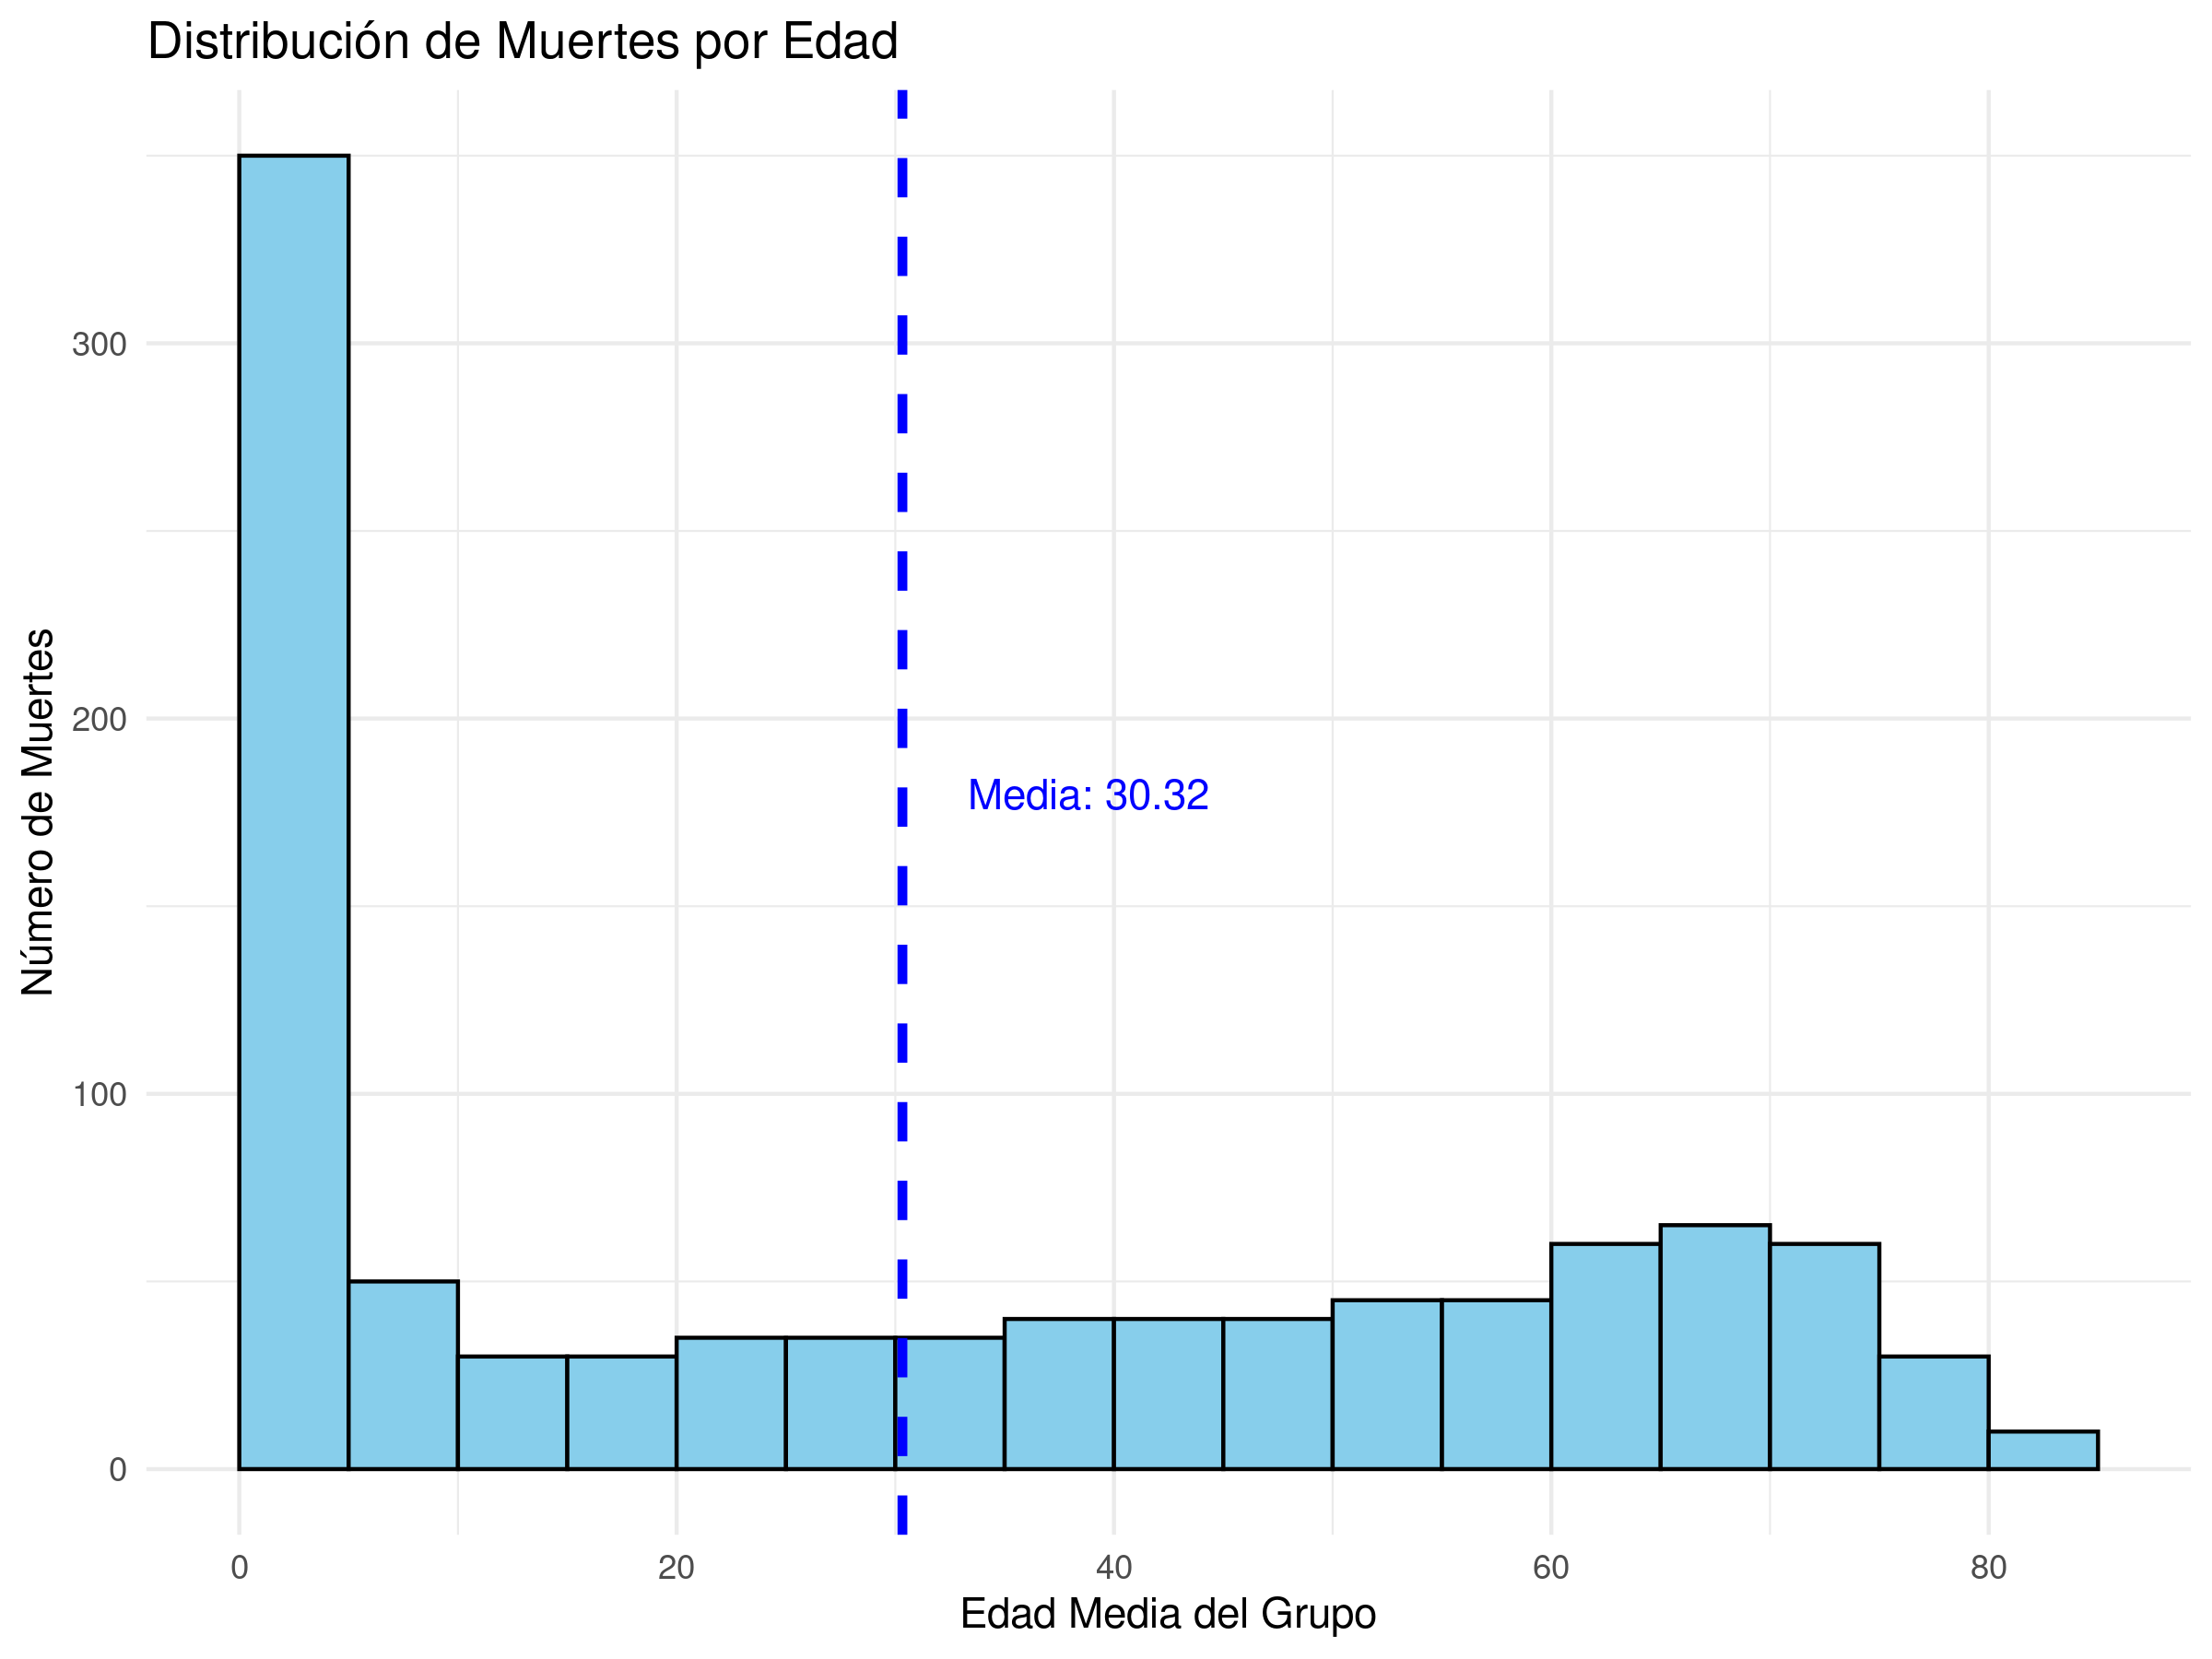
\includegraphics[width=0.8\linewidth]{img/distribucion_muertes.png}
        \caption{Gráfico obtenido de R.}
    \end{figure}

    \noindent
    Ahora sí que vemos lo que está pasando: resulta que en la Edad Media había muchísima mortalidad natal, por lo que una gran cantidad (de 1000 muertes, 350 se corresponden a personas de menos de 5 años) de personas no superaba los 5 años. Sin embargo, este hecho no tiene nada que ver con la calidad de vida de una persona que consigue superar esta mortalidad infantil, por lo que estamos tratando mal los datos: no se trata de una única variable aleatoria, tenemos una distribución bimodal como resultado de la suma de dos variables aleatorias: mortalidad infantil y esperanza de vida.\\

    \noindent
    La media solo hace un buen resumen de los datos cuando la distribución es unimodal. Así, lo que debíamos haber hecho al calcular la edad media de defunción es quedarnos solo con las personas de una edad en adelante. Este margen habría que estudiar bien dónde ponerlo pero parece que a partir de los 10 años esta mortalidad infantil deja de tener tanta relevancia:
    \begin{minted}{r}
# 1. Quedarme con los datos de personas mayores de 10 años
datos_filtrados <- datos[datos$Edad_Media >= 10, ]

# 2. Calcular la edad media ponderada por el número de muertes
media_filtrados_ponderada <- sum(datos_filtrados$Edad_Media * datos_filtrados$Muertes_dx) / sum(datos_filtrados$Muertes_dx)
media_filtrados_ponderada 
    \end{minted}
    Obtenemos \texttt{media\_filtrados\_ponderada = 49.125}, grafiquémoslo:
    \begin{minted}{r}
ggplot(datos, aes(x = Edad_Media, weight = Muertes_dx)) +
  geom_histogram(binwidth = 5, fill = "skyblue", color = "black", boundary = 0) +
  geom_vline(xintercept = media_ponderada, color = "blue", linewidth = 1.2, linetype = "dashed") +
  annotate("text", x = media_ponderada + 3, y = max(datos$Muertes_dx) * 0.9, 
           label = paste("Media:", round(media_ponderada, 2)), color = "blue", hjust = 0) +
  geom_vline(xintercept = media_filtrados_ponderada, color = "red", linewidth = 1.2, linetype = "dashed") +
  annotate("text", x = media_filtrados_ponderada + 3, y = max(datos$Muertes_dx) * 0.9, 
           label = paste("Media (>= 10):", round(media_filtrados_ponderada, 2)), color = "red", hjust = 0) +
  labs(
    title = "Distribución de Muertes por Edad",
    x = "Edad Media del Grupo",
    y = "Número de Muertes"
  ) +
  theme_minimal()
        
    \end{minted}
    \begin{figure}[H]
        \centering
        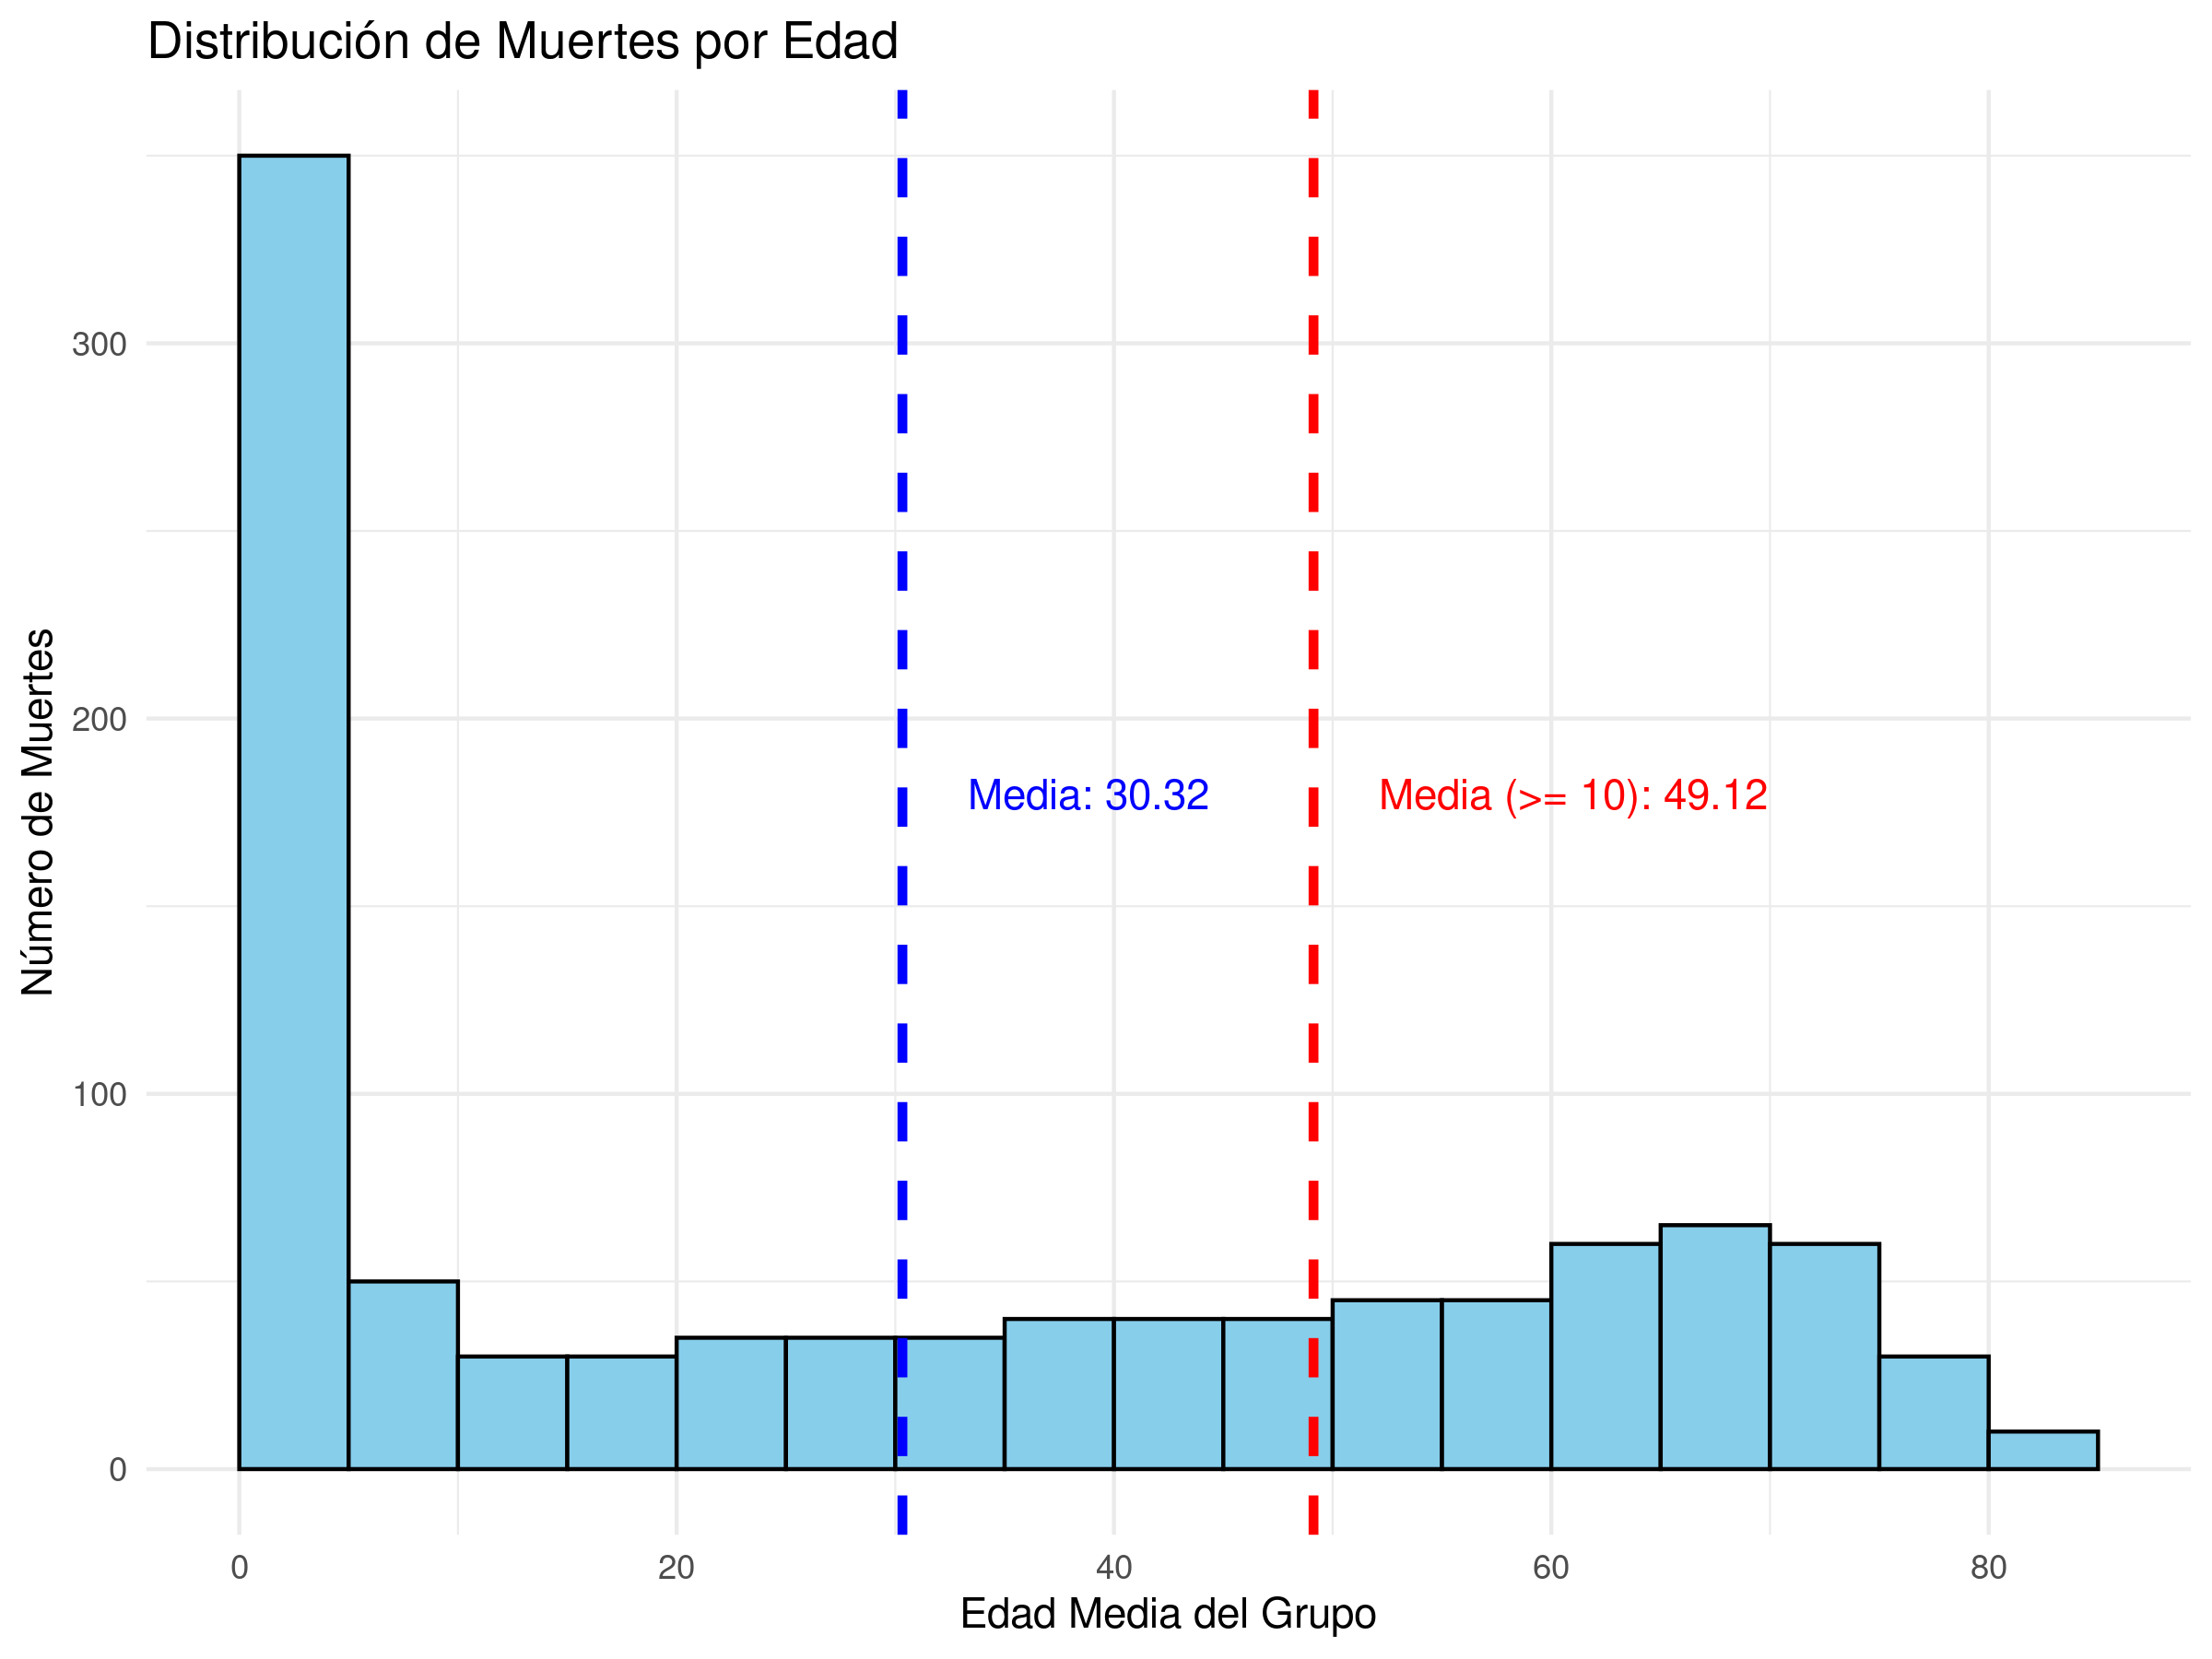
\includegraphics[width=0.8\linewidth]{img/distribucion_muertes2.png}
    \end{figure}
\end{ejemplo}

\section{Estadísticos}

\begin{definicion}
    Una medida se considera \textbf{resistente} si muestra poca sensibilidad frente a valores anómalos (\textit{outliers}).
\end{definicion}

\begin{ejemplo}
    Consideremos las dos siguientes distribuciones de datos experimentales:
    \begin{figure}[H]
        \centering
    \begin{tabular}{c|cc}
        Dato & Frecuencia Muestra 1 & Frecuecia Muestra 2 \\
        \hline
        10 & 2 & 2 \\
        11 & 1 & 1 \\
        12 & 2 & 2 \\
        13 & 1 & 1 \\
        14 & 1 & 1 \\
        15 & 3 & 3 \\
        16 & 1 & 1 \\
        17 & 0 & 0 \\
        18 & 1 & 1 \\
        19 & 1 & 0 \\
        20 & 0 & 0 \\
        \vdots & \vdots & \vdots \\
        57 & 0 & 1 
    \end{tabular}
    \caption{Datos experimentales.}
    \end{figure}

    \noindent
    Vemos que en los datos superiores parece que tenemos un \textit{outlier} en la segunda muestra, puesto que 57 parece ser un valor raro respecto al resto de valores.

    \noindent
    Si calculamos varias medidas estadísticas:
    \begin{table}[H]
    \centering
    \begin{tabular}{l|rr}
        Medida & Muestra 1 & Muestra 2 \\
        \hline
        $N$ & 13 & 13 \\
        Media & 13.8462 & 16.7692 \\
        Mediana & 14 & 14 \\
        Desv. típica & 2.8533 & 12.3231 \\
        Varianza & 8.141 & 151.859 \\
        Asimetría & 0.310 & 3.368 \\
        Curtosis & -0.688 & 11.774
    \end{tabular}
    \caption{Medidas estadísticas.}
    \end{table}

    \noindent
    Vemos que casi todas las medidas estadísticas se han modificado bastante, salvo la mediana, que ha permanecido igual, porque la mediana no está basada en frecuencias, sino en cuartiles. Podríamos decir que la mediana es una medida resistente.
\end{ejemplo}

\begin{definicion}
    Una medida se dice \textbf{robusta} si muestra poca sensibilidad frente al incumplimiento de hipótesis de partida en los modelos prababilísticos.
\end{definicion}

\subsection{Tipos de percentiles}
\noindent
Para una variable aleatoria $X$ con función de distribución $F$, se define para $p \in \left]0,1\right[$ su $p-$ésimo percentil como:
\begin{equation*}
    Q(p) = F^{-1}(p) = \inf\{x : F(x)\geq p\}
\end{equation*}
Si tenemos una muestra $X_1,\ldots,X_n$ de tamaño $n$, Hyndman y Fan realizaron una clasificación de los 9 tipos de percentiles que podemos considerar, clasificándolos en percentiles para variables discretas o para variables continuas. Todos estos percentiles tienen algo en común:
\begin{itemize}
    \item En primer lugar se calcula $np + m$, para $m$ una constante predefinida.
    \item Se toma $i = \lfloor np + m \rfloor$ la parte entera y $g = np + m - i$ la parte decimal.
    \item En función de los cálculos obtenidos se fija un valor de $\gamma$ y se toma:
        \begin{equation*}
            Q(p) = (1-\gamma) X_i + \gamma X_{i+1}
        \end{equation*}
\end{itemize}
Veamos todos los tipos de percentiles que podemos encontranos:
\subsubsection{Para variables discretas}
\begin{enumerate}
    \item Se toma $m=0$, por lo que $np = i + g$.
        \begin{itemize}
            \item Si $g=0$ se toma $\gamma=0$, es decir, $Q_1(p) = X_i$.
            \item Si $g\neq0$ se toma $\gamma=1$, es decir, $Q_1(p) = X_{i+1}$.
        \end{itemize}
        Este percentil se denomina \textbf{EMPIRICAL}.
    \item Se toma $m=0$, por lo que $np = i + g$.
        \begin{itemize}
            \item Si $g=0$ se toma $\gamma=0.5$, es decir, $Q_2(p) = 0.5(X_i + X_{i+1})$.
            \item Si $g\neq 0$ se toma $\gamma=1$, es decir, $Q_2(p) = X_{i+1}$.
        \end{itemize}
        Este percentil se denomina \textbf{AEMPIRICAL}.
    \item Se toma $m=-\frac{1}{2}$, por lo que $np - \frac{1}{2} = i+g$.
        \begin{itemize}
            \item Si $g=0$ y $i$ es impar se toma $\gamma=0$, es decir, $Q_3(p) = X_i$.
            \item Si $g\neq 0$ o $i$ es par se toma $\gamma=1$, es decir, $Q_3(p) = X_{i+1}$
        \end{itemize}
        Este percentil se denomina \textbf{SAS}, estadístico de orden más cercano.
\end{enumerate}
\subsubsection{Para variables continuas}
\begin{enumerate}
    \item[4.] Se toma $m=0$, por lo que $np = i+g$.

        En este caso se toma $\gamma=g$, con lo que:
        \begin{equation*}
            Q_4(p) = (1-g)X_i + gX_{i+1}
        \end{equation*}
        Este percentil se denomina \textbf{WAVERAGE}.
    \item[5.] Se toma $m=\frac{1}{2}$, por lo que $np + \frac{1}{2}=i + g$.
        \begin{itemize}
            \item Si $F(pn) < 0.5$ se toma $Q_5(p) = X_i$.
            \item Si $F(pn) \geq 0.5$ se toma $Q_5(p) = X_{i+1}$
        \end{itemize}
        Este percentil se denomina \textbf{ROUND}.
    \item[6.] Se toma $m=p$, por lo que $(n+1)p = i + g$.

        Se toma $\gamma = g$, con lo que:
        \begin{equation*}
            Q_6(p) = (1-g)X_i + gX_{i+1}
        \end{equation*}
        Este percentil se denomina \textbf{HAVERAGE-Tuckey}, es el por defecto en SPSS.
    \item[7.] Se  toma $m=1-p$, por lo que $(n-1)p+1 = i + g$.
        Se toma $\gamma = g$, con lo que:
        \begin{equation*}
            Q_7(p) = (1-g)X_i + gX_{i+1}
        \end{equation*}
        Este percentil es el por defecto en R y Excel.
    \item[8.] Se toma $m=\nicefrac{(p+1)}{3}$, por lo que $n+\frac{p}{3}+\frac{1}{3}=i+g$.
        Se toma $\gamma = g$, con lo que:
        \begin{equation*}
            Q_8(p) = (1-g)X_i + gX_{i+1}
        \end{equation*}
        Este percentil se denomina ``Insesgado respecto a la mediana''.
    \item [9.] Se toma $m=\frac{p}{4}+\frac{3}{8}$, por lo que $n+\frac{p}{4}+\frac{3}{8}=i+g$.
        Se toma $\gamma = g$, con lo que:
        \begin{equation*}
            Q_8(p) = (1-g)X_i + gX_{i+1}
        \end{equation*}
        Este percentil se denomina ``Insesgado para distribuciones normales''.
\end{enumerate}

\subsection{Medidas robustas de posición central}
\noindent
Las medidas que menos se influencian por datos anómalos son las medidas basadas en percentiles, puesto que muchos datos han de cambiar para que un percentil cambie. Veamos algunas de estas medidas:
\begin{description}
    \item [Mediana.] 
        \begin{equation*}
            Me = Q(0.5)
        \end{equation*}
    \item [Punto medio entre cuartiles.] 
        \begin{equation*}
            \overline{Q} = \frac{Q(0.25) + Q(0.75)}{2}
        \end{equation*}
        Esta medida puede ayudarnos a detectar si una distribución unimodal es simétrica o si presenta una acumulacióna izquierda o derecha:
        \begin{itemize}
            \item Si $Me < \overline{Q}$, entonces la distribución se acumula a la izquierda.
            \item Si $Me > \overline{Q}$, entonces la distribución se acumula a la derecha.
        \end{itemize}

        \begin{figure}[H]
        \centering
        \begin{tikzpicture}
        \begin{axis}[
            no markers,
            domain=0:10,
            samples=200,
            axis lines=left,
            xlabel={$x$},
            ylabel={$f(x)$},
            ymin=0, ymax=0.45,
            xmin=0, xmax=10.5,
            xtick=\empty,
            ytick=\empty,
            height=7cm, width=11cm,
            enlargelimits=false
        ]

            % Función de densidad asimétrica a la derecha (Basada en distribución Chi-cuadrado / Gamma)
            \addplot[name path=f, thick, black] {0.35 * x * exp(-x/1.8)};

            % Puntos de los cuartiles (calculados para esta curva)
            \pgfmathsetmacro{\qone}{1.73}   % Q(0.25)
            \pgfmathsetmacro{\qtwo}{2.98}   % Q(0.50) - Mediana
            \pgfmathsetmacro{\qthree}{4.85} % Q(0.75)

            % Sombreado de los cuatro cuartiles (Alternando colores suaves)
            \addplot[fill=blue!10, draw=none, domain=0:\qone] {0.35 * x * exp(-x/1.8)} \closedcycle;
            \addplot[fill=blue!20, draw=none, domain=\qone:\qtwo] {0.35 * x * exp(-x/1.8)} \closedcycle;
            \addplot[fill=blue!30, draw=none, domain=\qtwo:\qthree] {0.35 * x * exp(-x/1.8)} \closedcycle;
            \addplot[fill=blue!40, draw=none, domain=\qthree:10] {0.35 * x * exp(-x/1.8)} \closedcycle;

            % Rediseñar la curva por encima para que no la tape el relleno
            \addplot[thick, black] {0.35 * x * exp(-x/1.8)};

            % Líneas verticales para los cuartiles
            \draw[dashed, thick, black!70] (axis cs:\qone,0) -- (axis cs:\qone,{0.35 * \qone * exp(-\qone/1.8)});
            \draw[thick, black!70] (axis cs:\qtwo,0) -- (axis cs:\qtwo,0.25);
            \draw[dashed, thick, black!70] (axis cs:\qthree,0) -- (axis cs:\qthree,{0.35 * \qthree * exp(-\qthree/1.8)});

            \fill (\qone,0.23) node[above] {$Q(0.25)$};
            \fill (\qtwo,0.25) node[above] {$Me$};
            \fill (\qthree,0.11) node[above right] {$Q(0.75)$};

            \draw[dashed, black!70] (axis cs:3.29,0) -- (axis cs:3.29,0.23);
            \fill (3.29,0.23) node[right] {$\overline{Q}$};

            % Porcentajes dentro de cada área (25% cada una)
            \node at (axis cs:1.0, 0.08) {\small 25\%};
            \node at (axis cs:2.3, 0.12) {\small 25\%};
            \node at (axis cs:3.7, 0.10) {\small 25\%};
            \node at (axis cs:6.0, 0.04) {\small 25\%};
        \end{axis}
        \end{tikzpicture}
        \caption{Función de densidad con asimetría, división por cuartiles y punto medio entre cuartiles.}
        \end{figure}
        
    \item [Trimedia.] 
        \begin{equation*}
            TRI = \frac{Me+\overline{Q}}{2}
        \end{equation*}
    \item [Cuatrimedia.] Es la media aritmética considerando solo los valores que se encuentran contenidos estrictamente entre el primer y el tercer cuartil, es decir, esta medida no tiene en cuenta el 25\% de los datos más pequeños y el 25\% de los datos más grandes.
\end{description}
\subsection{Medidas robustas de dispersión}
\begin{description}
    \item [Rango intercuartílico.] 
        \begin{equation*}
            RIQ = Q(0.75) - Q(0.25)
        \end{equation*}
    \item [MEDA.] Es la MEdiana de las Desviaciones Absolutas respecto a la mediana.
    \item [Coeficiente de variación cuartílico.]
        \begin{equation*}
            CVc = \frac{\nicefrac{RIQ}{2}}{\overline{Q}} = \frac{Q(0.75)-Q(0.25)}{Q(0.75)+Q(0.25)}
        \end{equation*}
\end{description}
\subsection{Medidas robustas de forma}
\begin{description}
    \item[Coeficiente de Asimetría de Yule.]
        \begin{equation*}
            H_1 = \frac{Q(0.9)+Q(0.1) - 2Me}{Q(0.9)-Q(0.1)} = \frac{\overline{Q}}{Me} - 1
        \end{equation*}
        La interpretación es la vista en la figura anterior:
        \begin{itemize}
            \item Si $H_1=0$ la distribución es simétrica.
            \item Si $H_1>0$ la distribución es asimétrica a la derecha.
            \item Si $H_1<0$ la distribución es asimétrica a la izquierda.
        \end{itemize}
    \item[Coeficiente de Asimetría de David y Johnson.]
        \begin{equation*}
            H_2(\alpha) = \frac{\overline{Q}(\alpha) - Me}{\frac{RIQ(\alpha)}{2}}
        \end{equation*}
    \item[Coeficiente de Asimetría de Kelly.]
        \begin{equation*}
            H_3 = \frac{Q(0.9)+Q(0.1) - 2Me}{Q(0.9)-Q(0.1)}
        \end{equation*}
\end{description}

% Gráfica de centiles y (v,u)  de variables discretas

\section{Construcción de disgrama de cajas con bigotes}
\noindent
Para una muestra de una variable aleatoria $X$ de tamaño $N$ usaremos el percentil tipo 6, o de HAVERAGE-Tuckey. Los pasos para construir una caja con bigotes son:
\begin{itemize}
    \item Se representa la caja de modo que el extremo inferior de la misma se corresponda con el primer cuartil de Tuckey $T_1$ y que el extremo superior se corresponda con el tercer cuartil $T_3$.

        Posteriormente, se dibuja una línea dentro de la caja que se corresponde con la mediana $Me$.
    \item Los bigotes se construyen uniendo una línea desde el centro de la caja con el último (equivalementente, primer) valor de la distribución que esté a una distancia máxima de un $RIQ = T_3 - T_1$.
    \item Los valores que se encuentran fuera de estos bigotes y a distancia máxima de $1.5 RIQ$ se marcan individualmente.
    \item Un valor a distancia entre $1.5RIQ$ y $3RIQ$ se considera un valor alejado, o \textit{outside}.
    \item Una valor a mayor distancia que $3RIQ$ se considera extremadamente alejado, o \textit{far outside}.
\end{itemize}

\begin{ejercicio}
    Demostrar:
    \begin{enumerate}
        \item Si $Z\rightsquigarrow\cc{N}(0,1)$, entonces:
            \begin{equation*}
                P[Q_1-RIQ\leq Z \leq Q_3 + RIQ] \geq 0.95
            \end{equation*}
        \item Lo anterior es cierto para $X\rightsquigarrow\cc{N}(\mu, \sigma^2)$
    \end{enumerate}
    Hagamos este ejercicio:
    \begin{enumerate}
        \item Tenemos que calcular entonces:
            \begin{equation*}
                P[Q_1-RIQ\leq Z\leq Q_3+RIQ]
            \end{equation*}
            Para ello, como $\cc{N}(0,1)$ es una distribución simétrica tenemos que calcular simplemente:
            \begin{equation*}
                P[Q_1-RIQ\leq Z] = P[Q_1-Q_3+Q_1\leq Z] \AstIg P[3Q_1\leq Z]
            \end{equation*}
            donde en $(\ast)$ hemos usado que $Q_3 = -Q_3$ por ser la distribución simétrica.\\

            \noindent
            Consultamos el valor de $Q_1$ en la tabla de la normal $\cc{N}(0,1)$, buscamos el menor $x$ con $P[x\leq Z] \geq 0.25$, obteniendo aproximadamente $Q_1 = -0.68$. Ahora hemos de calcular $(3\cdot 0.68 = 2.04):$
            \begin{equation*}
                P[3Q_1 \leq Z] \approx P[-2.04 \leq Z] = P[Z\leq 2.04] \approx 0.9793 
            \end{equation*}
            Así, tenemos ahora que:
            \begin{align*}
                P[Q_1-RIQ\leq Z\leq Q_3+RIQ] &= 1 - 2\cdot P[Z\leq Q_1-RIQ] \\
                                             &= 1 - 2(1-P[Z\geq Q_1-RIQ]) \\
                                             &= -1 + 2P[Z\geq Q_1-RIQ] \\
                                             &\approx -1 + 2\cdot 0.9793 = 0.9586
            \end{align*}
        \item De la tipificación de las variables normales:
            \begin{equation*}
                Z = \frac{X-\mu}{\sigma}
            \end{equation*}
            obtenemos que:
            \begin{equation*}
                Q_1(Z) = \frac{Q_1(X)-\mu}{\sigma}
            \end{equation*}
            Por lo que es trivial que:
            \begin{equation*}
                P[Q_1(X)-RIQ(X)\leq X\leq Q_3(X)+RIQ(X)] \geq 0.95
            \end{equation*}
    \end{enumerate}
\end{ejercicio}

\begin{ejercicio}
    Calcular la probabilidad de que un punto de una distribución $\cc{N}(0,1)$ sea un \textit{outside} o un \textit{far outside}.
\end{ejercicio}
